\section{Réseaux siamois}
\subsection{Généralités}
Les réseaux siamois\cite{siamese} constituent une famille d'architectures formées de deux (ou plus) sous-réseaux identiques, i.e même configuration avec des paramètres et poids identiques. Lors de l'apprentissage, les sous-réseaux sont mis à jour de manière identique. La nature des architectures des sous-réseaux est variable (convolutif, récurrent, Full-Connected...) et dépend de la nature des données à analyser. Ce réseau est composé de deux parties:
\begin{itemize}
    \item \textbf{Extraction d'attributs}: Cette tâche est réalisée par les sous-réseaux qui vont représenter la donnée d'entrée sous la forme d'un vecteur d'attribut résumant l'information portée. Les sous-réseaux étant identiques, le comportement des extracteurs est identique peu importe la donnée analysée (donnée de référence et donnée à analyser). Ainsi, dans le cas de la reconnaissance faciale, les deux visages à comparer seront représentés par un vecteur définissant les attributs physiques des deux individus.
    \item \textbf{Mesure de similarité}: Cette tâche est réalisée par une métrique de distance qui évalue la similarité entre deux vecteurs d'attributs. On peut citer la \textit{Mean Squared Error} et la \textit{Distance Cosinus} par exemple\footnote{Il existe de nombreuses autres métriques utilisables !}. La sortie est donc une valeur comprise entre 0 et 1 qui détermine le degrés de similarité entre deux entités.\\

    Néanmoins, ce type de métrique est peu effective dans les faits car elle favorise des convergences peu effectives, notamment en tolérant que les valeurs de sortie des entités jugées similaires et dissimilaires soient "proches". Il est préférable de favoriser un écart important entre les résultats positifs et négatifs, i.e imposer une \textit{marge}. Cette particularité est réalisé par la \textit{Contrastive Loss function}\cite{contlossfn}\footnote{Il existe aussi des métriques qui respecte cette condition en ne se basant pas sur une marge}. Soit $\vec{X_i}$, une valeur d'entrée et $G(\vec{X_i})$, la sortie obtenue après action d'un sous-réseau et y, valeur binaire de prédiction. \textit{Contrastive Loss function}\footnote{On supposera qu'une similarité parfaite équivaut à un résultat de 0} est ainsi définie\footnote{Voir la Section \ref{tripletloss} pour plus de détails sur la notion de marge.} par:
    $$(1-y)*\frac{1}{2}D_w^2(\vec{X_1},\vec{X_2})+y*\frac{1}{2}(max(0, m-D_w(\vec{X_1},\vec{X_2})))^2$$
    $$D_w(\vec{X_1},\vec{X_2})=||G(\vec{X_1})-G(\vec{X_2})||_2$$
\end{itemize}

\noindent Un exemple de réseau siamois est visible sur la Figure \ref{siamfig}. Les sous-réseaux suivent une architecture Full-connected. Les vecteurs caractéristiques sont dans $R^2$.\\

\begin{figure}
    \centering
    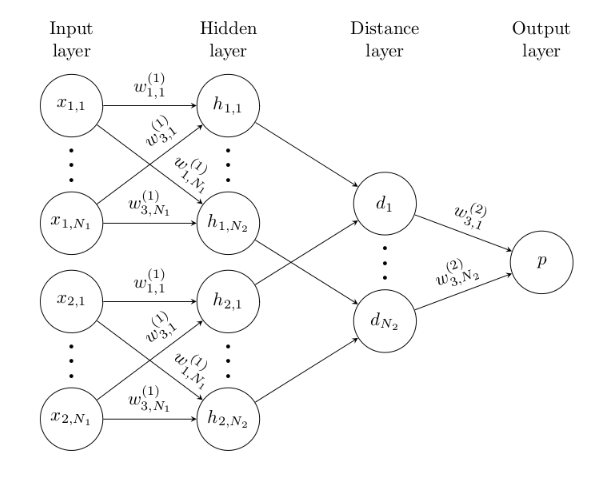
\includegraphics[scale=0.3]{./tex/siamese-network/siamepic.png}
    \caption{Exemple simple d'un réseau siamois}
    \label{siamfig}
\end{figure}

\noindent L'objectif de ce type de réseau est d'évaluer la similarité entre deux entités, ce qui s'oppose avec la tâche classique des réseaux de neurones qui classifient une entité. De nombreux problèmes nécessitent une comparaison entre deux entités (peu importe si le réseau est capable de les classifier), notamment la reconnaissance faciale (\textit{Face Recognition)}, de signature ou encore, d'écriture (par rapport au style graphique si écrit à la main ou au style syntaxique). Plus récemment, de nouvelles thématiques ont été abordées telles que l'évaluation de la pertinence d'une réponse à une question donnée\footnote{Approche très utile dans le cadre d'un apprentissage d'un ChatBot} ou encore le \textit{Tracking}. Ce type de réseau est très exploité dans le domaine du \textbf{One-Shot Learning}.\\

\subsection{Triplet Loss}
\label{tripletloss}
Une autre fonction populaire - comparable à la \textit{Contrastive Loss function} - est la \textit{Triplet Loss}\cite{tripletloss}. La \textit{Contrastive Loss function} cherche à minimiser la distance si les deux images sont de la même classe et à maximiser (associer une valeur supérieure à une marge) si les deux images sont de classes différentes. Cette métrique considère des couples d'entités et réalise sa discrimination en fonction de la concordance des entités de ce couple. Ainsi, elle maximise (ou minimise) les distances entre entités de manière dissociées.\\

\noindent Au contraire, \textit{Triplet Loss} exploite des triplets d'entités (A,P,N) avec A, image de référence, P, image positive (de même classe) et N, image négative (de classe différente). L'objectif de cette métrique est de permettre que la projection de l'image positive soit plus "proche" de la référence que l'image négative, i.e maximiser la différence entre (A-N) et (A-P). Cette approche considère ainsi les distances de manière \textit{relative}. En effet, sa référence est basée sur la différence entre (A-N) et (A-P) et non des distances \textit{absolues}. Cette métrique est donc plus \textit{laxiste} car elle ne forcera pas la réduction de distance qui peut être trop exigeante. Par exemple, dans le cas de la \textit{Contrastive Loss function}, l'apprentissage va chercher à diminuer au maximum la distance entre deux entités similaires alors que dans le cas de \textit{Triplet Loss}, l'apprentissage se limitera à garantir une bonne séparation entre les entités similaires et dissimilaires. La condition est donc moins stricte.\\

\noindent Supposons un triplet (A,P,N). Nous voulons faire en sorte que l'image positive soit plus proche de la référence que l'image négative. Supposons f, la fonction de transformation des sous-réseaux. Ainsi, nous obtenons:
$$\underbrace{||f(A)-f(P)||_2}_{D(A,P)} \leq \underbrace{||f(A)-f(N)||_2}_{D(A,N)}$$
$$\underbrace{||f(A)-f(P)||_2}_{D(A,P)} - \underbrace{||f(A)-f(N)||_2}_{D(A,N)}\leq 0 \ \ \ \ \ \ (1)$$
\noindent Cette approche présente une faiblesse majeure. En effet, la condition tolère le cas où:
$$D(A,P) \longrightarrow 0$$
$$D(A,N) \longrightarrow 0$$
\noindent Pour contrer ce phénomène, on instaure une \textit{marge} qui forcera un éloignement des projections des entités négatives. Ainsi, nous obtenons:
$$D(A,P) + \alpha \leq D(A,N)$$
$$D(A,P) - D(A,N) + \alpha \leq 0\ \ \ \ \ \ (2)$$
\noindent Supposons un exemple. Si on utilise l'équation (1), si D(A,P)=0.3 et D(A,N)=0.33, alors la condition est remplie. Néanmoins, la discrimination est très faible et le risque de faux-positif et faux-négatif élevé à cause de cette proximité. Supposons l'équation (2) si D(A,P)=0.3 et $\alpha=0.3$ alors il faut que $D(A,N) \geq 0.6$ pour que la condition soit satisfaite, ce qui favorise une discrimination importante.\\

\noindent Il reste à formaliser cette condition afin de la rendre exploitable par un réseau de neurones. Nous pouvons réecrire l'équation (2) telle que pour un triplet (A,P,N):
$$\mathcal{L}(A,P,N)=max(\underbrace{||f(A)-f(P)||_2}_{D(A,P)} - \underbrace{||f(A)-f(N)||_2}_{D(A,N)}+\alpha,0) $$
$$\mathcal{L}(minibatch_{(A,P,N)})=\sum_{i=1}^n \mathcal{L}(A^{(i)},P^{(i)},N^{(i)})$$

\noindent \textbf{Attention}: Si les triplets (A,P,N) sont choisis aléatoirement, la condition peut être facilement satisfaite et nuire à la performance du modèle du fait de l'apprentissage trop "facile". Il est important de créer des triplets "difficiles" à entraîner en utilisant des entités qui se "ressemblent" !
